% IPEC2026.cls is based on IEEEtran.cls.
% Please read the instructions for IEEEtran.cls before using IPEC2026.cls.
\documentclass{IPEC2026}
%\IEEEoverridecommandlockouts
% The preceding line is only needed to identify funding in the first footnote. If that is unneeded, please comment it out.
\usepackage{cite}
\usepackage{amsmath,amssymb,amsfonts}
\usepackage{algorithmic}
\usepackage{graphicx}
\usepackage{textcomp}
\usepackage{xcolor}
\usepackage{url} 
\def\BibTeX{{\rm B\kern-.05em{\sc i\kern-.025em b}\kern-.08em
    T\kern-.1667em\lower.7ex\hbox{E}\kern-.125emX}}
%s\usepackage{tikz}
\usepackage{pgfplots}
\pgfplotsset{compat=1.18}
\usepackage[font={footnotesize}]{caption}          % Necessary for subcaption
\usepackage{subcaption}       % Multiple figures in one
\usepackage{tabularx}
\usepackage{tabularray}
\UseTblrLibrary{booktabs}

\usepackage{siunitx}                % Units; e.g. prevents linebreak between number and unit
\sisetup{
  per-mode=symbol-or-fraction,
  output-exponent-marker=\ensuremath{\mathrm{e}},
  range-units = single  % Use 1 to 3 MHz instead of 1 MHz to 3 MHz
  %fraction-function=\tfrac
}
\DeclareSIUnit{\inch}{in}

% Adjust the spacing around a figure
% 8pt plus 1pt minus 2pt: a “rubber length” with base = 8pt; stretch = up to +1pt (can grow to 9pt if there’s extra space); shrink = up to −2pt (can shrink to 6pt if the page is tight)
\setlength{\textfloatsep}{4pt plus 3pt minus 1pt}    
% Space above/below display equations
\setlength{\abovedisplayskip}{6pt plus 3pt minus 1pt}  
\setlength{\belowdisplayskip}{6pt plus 3pt minus 1pt} 
% “Short” variants used when the preceding line is short or ends with a display trigger
\setlength{\abovedisplayshortskip}{5pt plus 3pt minus 1pt}
\setlength{\belowdisplayshortskip}{5pt plus 3pt minus 1pt}

\usepackage[acronym]{glossaries}
% Just for having less to type
\newcommand{\sbl}[1]{\glssymbol{#1}}
% To allow compatibility with acronym package syntax, define \ac
\newcommand{\ac}{\gls}
\newcommand{\acp}{\glspl}

\newcommand{\mathSymbol}[3]{
    \newglossaryentry{#1}{symbol={\ensuremath{#2}}, name={#3}, description={}, sort={#1}}
}

\mathSymbol{Lself}{L_\mathrm {self}}{Self-inductance of each coil of a symmetrical coupled inductor}
\mathSymbol{k}{k}{Coupling-factor of the coupled inductor}
\mathSymbol{Lm}{L_\mathrm m}{Magnetizing inductance in the transformer model}
\mathSymbol{Lout}{L_\mathrm {out}}{Output inductance in the transformer model}
\mathSymbol{im}{i_\mathrm m}{Magnetizing current in the transformer model}
\mathSymbol{iout}{i_\mathrm {out}}{Output current}
\mathSymbol{v1}{v_\mathrm 1}{Voltage at the switch-node leg 1}
\mathSymbol{v2}{v_\mathrm 2}{Voltage at the switch-node leg 2}
\mathSymbol{i1}{i_\mathrm 1}{Current of leg 1}
\mathSymbol{i2}{i_\mathrm 2}{Current of leg 2}
\mathSymbol{vout}{v_\mathrm {out}}{Output voltage}
\mathSymbol{Ts}{T_\mathrm s}{Switching period}
\mathSymbol{fs}{f_\mathrm s}{Switching frequency}
\mathSymbol{Deff}{D_\mathrm {eff}}{Effective duty cycle}
\mathSymbol{D}{D}{Duty cycle}
\mathSymbol{Vin}{V_\mathrm {in}}{Input voltage}
\mathSymbol{DeltaIleg}{\Delta I_\mathrm {leg}}{Peak-to-peak leg current ripple}
\mathSymbol{DeltaIout}{\Delta I_\mathrm {out}}{Peak-to-peak output current ripple}
\mathSymbol{Ion}{I_\mathrm {on}}{Turn-on current}
\mathSymbol{Ion,max}{I_\mathrm {on,max}}{Maximum turn-on current}
\mathSymbol{Hdc}{H_\mathrm {dc}}{DC field strength}
\mathSymbol{mui}{\mu _\mathrm i}{Initial Permeability}
\mathSymbol{Pout}{P_\mathrm {out}}{Output Power}
\mathSymbol{Cin}{C_\mathrm {in}}{Input capacitance}
\mathSymbol{Cout}{C_\mathrm {out}}{Output capacitance}

\newacronym{tcm}{TCM}{triangular current mode}
\newacronym{zvs}{ZVS}{zero voltage switching}
\newacronym{pcb}{PCB}{printed circuit board}
\newacronym{gan}{GaN}{Gallium Nitride}

\begin{document}

\title{Novel Single-Turn Coupled-Inductor with MHz-Range Operation in Triangular Current Mode for 48 to 12 V conversion
%\thanks{Identify applicable funding agency here. If none, delete this.}
}
%Optimized Design of a Coupled-Inductor Buck Converter, 48 to 12 V, 1 kW, Using Planar Magnetics and GaN-FETs for MHz-Range Operation


% Please replace * with your track number
\track{6. Vehicle Electrification-related Technologies}

%Class IPEC2026: The \author command is disabled in this template.

\maketitle

\begin{abstract}
The next generation of automotive vehicles and datacenters requires highly compact and efficient 48 V to 12 V point-of-load converters. This paper presents a novel single-turn planar inductor geometry with four poles and dual air-gap for operation beyond 1 MHz that minimizes copper-losses from external proximity effect. An experimental prototype with 1 kW output achieves an impressive power density of 80 kW/l (1300 W/in³) and a peak efficiency of 96.3\%, demonstrating the potential of the inductor structure.
\end{abstract}

\begin{IEEEkeywords}
automotive 48 V to 12 V, coupled inductor, high power density, soft-switching
%The authors shall provide up to 4 keywords or phrases (in alphabetical order and separated by commas) to help identify the major topics of the paper.
\end{IEEEkeywords}

\section{Introduction}
With a growing power demand, power distribution in both conventional and electric vehicles presents an increasing challenge. Traditionally, \qty{12}{\V} are used to distribute the power to all auxiliary devices which requires large cable diameters. Moving to a \qty{48}{\V} distribution bus reduces the cost of the wire assembly and losses \cite{kumawatComprehensiveStudyAutomotive2019}. As most devices are still operating at \qty{12}{\V}, highly compact and efficient point-of-load converters are required. This conversion stage is a critical part of distributed power architectures and its performance has a direct impact on system-level efficiency, thermal design, and overall build volume \cite{kumawatComprehensiveStudyAutomotive2019}. With the rise of \ac{gan} power devices, operating converters in the MHz-range has become feasible, significantly reducing their size \cite{weitzHighFrequencyResonant2023}. Resonant converters with planar transformers are a common choice but are unsuitable when a regulated output voltage is required over a wide input voltage range. The classical buck converter is suited well for those cases but the design of compact and efficient planar inductors is challenging due to the missing possibility for interleaving, the fringing of the air-gap, and the DC-bias in the core. \par
%Utilizing multi-phase converters with coupled inductors is an effective way to reduce the volume and loss of the planar inductors as the flux can cancel out in certain areas \cite{huaUltrathinCoupledInductor2021}. \par
In this paper, a \qty{1}{\kW} 2-phase coupled inductor buck converter for \qtyrange{48}{12}{\V} conversion is studied. To minimize the overall volume, a target switching-frequency range of \qtyrange{1}{3}{\MHz} was selected. Compared to previous work \cite{nan1MHzBidirectional2016, dongInvestigationMultiphaseCoupledInductor2009, shaZVSInterleavedSynchronousBuck2022, huaUltrathinCoupledInductor2021, wangPCBWindingBasedCoupled2023}, the low operating voltage requires a very low inductance whose design becomes particularly challenging due to the large phase current of \qty{40}{\A} with \qty{100}{\A} of ripple (required to achieve soft-switching). Firstly, the effects of coupling on the electrical parameters are analyzed mathematically. Afterwards, different geometries for the single-turn inductor are optimized using a novel winding geometry and dual air-gaps. The most promising geometry based on the four-pole structure is implemented and tested in an experimental prototype. %which achieves an impressive power density of 80 kW/l (1300 W/in³) and a peak efficiency of \qty{96.3}{\percent}, demonstrating the efficacy of the novel inductor structure.

%This motivates the use of wide-bandgap semiconductors which offer lower $R_{ds,on}$ and faster switching speeds compared to traditional Si-devices. By increasing the switching frequency, magnetic components and filters can be shrunk significantly enabling very high power densities. Beyond \qty{500}{\kHz} hard-switched converters are generally unsuitable due to their large switching losses CITE. A lot of research has been done on resonant converters as they inherently operate in soft-switching yielding high efficiencies and compact designs. However, those are unsuitable when a regulated output voltage is required over a wide input voltage range CITE. \par

% 28.7mm x 45.35mm x 9.8mm = 12.2cm3

%Soft-switching is maintained across all load conditions using Triangular Current Mode (TCM). GaN-FETs are employed to achieve fast switching transitions and low gate-drive losses but demand precise dead-time control to minimize reverse conduction losses. Conventionally, this requires expensive characterization across all operating conditions. To address this challenge, a novel circuit is proposed that monitors the reverse conduction duration in real-time, enabling dynamic dead-time optimization. First test results prove the desired operation of this circuit. Testing is still ongoing and currently the design is tested up to \qty{800}{\W} reaching a peak efficiency of \qty{95}{\percent} between 350 and \qty{600}{\W}. Multiple potential sources of unwanted losses have been identified and are currently investigated; efficiency is expected to significantly increase with small design changes. \\ Overall, this thesis shows that high-frequency interleaved buck converters with planar coupled inductors are a viable solution for point-of-load applications.

%The design of the inductor becomes a real challenge in the \unit{\MHz}-range as proximity and skin-effect play a significant role and increase copper losses drastically. A custom coupled inductor using planar magnetics was developed to cope with that. Through the combination of \acp{ganfet}, the custom inductor and soft-switched operation the converter pushes the boundaries of power density and efficiency.

\section{Coupled inductor buck converter in TCM}
\paragraph{Working principle}
\begin{figure} [b]
  \centering
  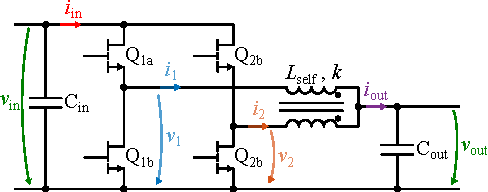
\includegraphics[width=0.9\columnwidth]{figures/Inkscape/Schematic.pdf}
  \caption{Schematic of the Coupled Inductor Buck Converter.}
  \label{fig:Schematic_BuckConfig_Coupled}
\end{figure}
The topology of the two phase coupled-inductor buck converter is shown in Fig. \ref{fig:Schematic_BuckConfig_Coupled}. It operates like a conventional two-phase buck with both legs are switched \qty{180}{\degree} out of phase. When the leg 2 is pulled high, the current in leg 1 is also affected as shown in Fig. \ref{fig:waveform_Coupling}: For positive coupling, the falling slope is steepened while for negative coupling it is flattened. The converter operates at very high ripple, more than twice the phase current. The low-side switch is kept on for a short period of time after the zero-crossing of the leg current such that the current becomes negative prior to the rising edge of each leg resulting in a \ac{zvs} turn-on of all transistors. This mode is commonly called \ac{tcm} \cite{marxgutInterleavedTriangularCurrent2010}. Only the small turn-off losses are observed now. If the dead-time is too long, the devices enter reverse-conduction creating additional losses. In practice, these reverse-conduction losses can be almost eliminated by properly adjusting the dead-time. %As the output current changes, the frequency needs to be adjusted to maintain the desired negative current.

\begin{figure}
  \begin{subfigure}[c]{0.51\columnwidth}
      \centering
      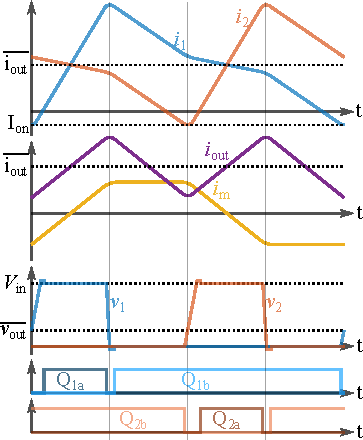
\includegraphics[width=\textwidth]{figures/Inkscape/Waveforms_negative.pdf}
      \subcaption{Negative Coupling}
      \label{fig:waveform_negCoupling}
    \end{subfigure}
    \begin{subfigure}[c]{0.48\columnwidth}
      \centering
      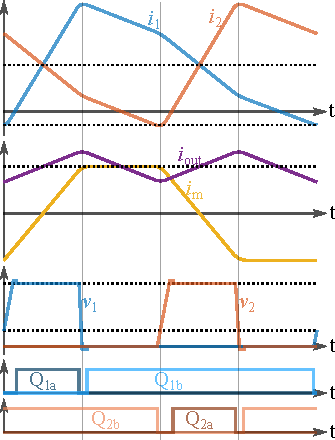
\includegraphics[width=\textwidth]{figures/Inkscape/Waveforms_positive.pdf}
      \subcaption{Positive Coupling}
      \label{fig:waveform_posCoupling}
    \end{subfigure}
  \caption{Waveforms for positive and negative coupling; dead-times are exaggerated. It can be seen that the slopes are changed but the behavior in the vicinity of the switching instances is fundamentally the same.}
  \label{fig:waveform_Coupling}
\end{figure}

\paragraph{Impact of the Coupling Factor}
\begin{figure}
  %\includegraphics[page=4, trim = 0cm 13.5cm 20cm 0cm, clip, width=\columnwidth]{figures/IPEC_Figures_PowerPoint.pdf}
  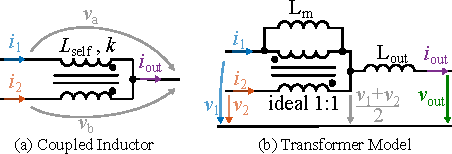
\includegraphics[width=0.9\columnwidth]{figures/Inkscape/Transformer-Model.pdf}
  \caption{The coupled inductor can be described with a self-inductance \sbl{Lself} and coupling factor \sbl{k} or by using an equivalent circuit consisting of an ideal 1:1 transformer with magnetizing inductance \sbl{Lm} and common output inductance \sbl{Lout}.}
  \label{fig:InductorModel}
\end{figure}
The symmetrical coupled inductor consists of two identical coils that are wound in a way, that the flux of one coil links with the flux of the second coil and vice versa with both coils connected on one side. This configuration can be described mathematically using 
\begin{equation}
  \label{eq:StandardCoupling}
  \begin{bmatrix} v_\mathrm a \\ v_\mathrm b \end{bmatrix} = \begin{bmatrix} 1 & \sbl{k} \\ \sbl{k} & 1 \end{bmatrix} \sbl{Lself} \begin{bmatrix} \frac{d\sbl{i1}}{dt}  \\ \frac{d\sbl{i2}}{dt} \end{bmatrix}
\end{equation}
with self-inductance \sbl{Lself} and coupling-factor \sbl{k}. Note that \sbl{k} can be positive or negative.
In order to provide a more intuitive understanding, the equivalent circuit in Fig. \ref{fig:InductorModel} (b) is introduced. Both circuits are electrically equivalent for $\sbl{Lout} = (1+\sbl{k})\frac{\sbl{Lself}}{2}$ and $\sbl{Lm} = (1-\sbl{k})\frac{\sbl{Lself}}{2}$.
The voltage at the virtual central node in the transformer model is only dependent on the two leg voltages \sbl{v1} and \sbl{v2}, decoupling the governing equations:
\begin{equation}
  \label{eq:TransformerModel}
  \begin{aligned}
    \frac{d\sbl{iout}}{dt} &= \frac{1}{\sbl{Lout}} \left (\frac{\sbl{v1} + \sbl{v2}}{2}-\sbl{vout} \right ) \\
    \frac{d\sbl{im}}{dt} &= \frac{1}{\sbl{Lout}} \left (\frac{\sbl{v1} - \sbl{v2}}{2} \right ) \\
    \text{with} \quad \sbl{iout} &= \sbl{i1} + \sbl{i2} \quad \text{and} \quad \sbl{im} = \sbl{i1} - \sbl{i2}
  \end{aligned}
\end{equation}
From this, the differential equations for each interval can be easily calculated and equations for the important converter parameters can be derived. An effective duty cycle \sbl{Deff} is introduced with $\sbl{Deff} = D$ for $\sbl{D} \leq 0.5$ and $\sbl{Deff} = 1-D$ for $\sbl{D} > 0.5$ to create universal equations. The peak-to-peak output ripple is then given by
\begin{equation}
  \sbl{DeltaIout} = \frac{2\sbl{Vin}}{\sbl{fs}(1+\sbl{k})\sbl{Lself}}\sbl{Deff}\left (\frac{1}{2}-\sbl{Deff} \right ).
  \label{eq:DeltaIout}
\end{equation}
The peak-to-peak ripple in each leg which is important for soft-switching is
\begin{equation}
  \sbl{DeltaIleg} =  \frac{\sbl{Vin}\sbl{Deff}}{2\sbl{fs}\sbl{Lself}} \left (\frac{2}{1+\sbl{k}} \left (\frac{1}{2}-\sbl{Deff} \right ) + \frac{1}{1-\sbl{k}} \right ).
  \label{eq:DeltaIleg}
\end{equation}

\sbl{Ion} needs to be below a certain negative value \sbl{Ion,max} to guarantee a sufficiently short dead time. This is fulfilled for
\begin{equation}
    \sbl{fs} < \frac{\sbl{Vin}\sbl{Deff}}{2\sbl{Lself}(\overline{\sbl{iout}}+2\sbl{Ion,max})} \left (\frac{2}{1+\sbl{k}}\left (\frac{1}{2}-\sbl{Deff} \right ) + \frac{1}{1-\sbl{k}} \right ).
    \label{eq:ConditionZVS}
\end{equation}

\section{Inductor Design}
\paragraph{Inductor geometry}
\begin{figure}
  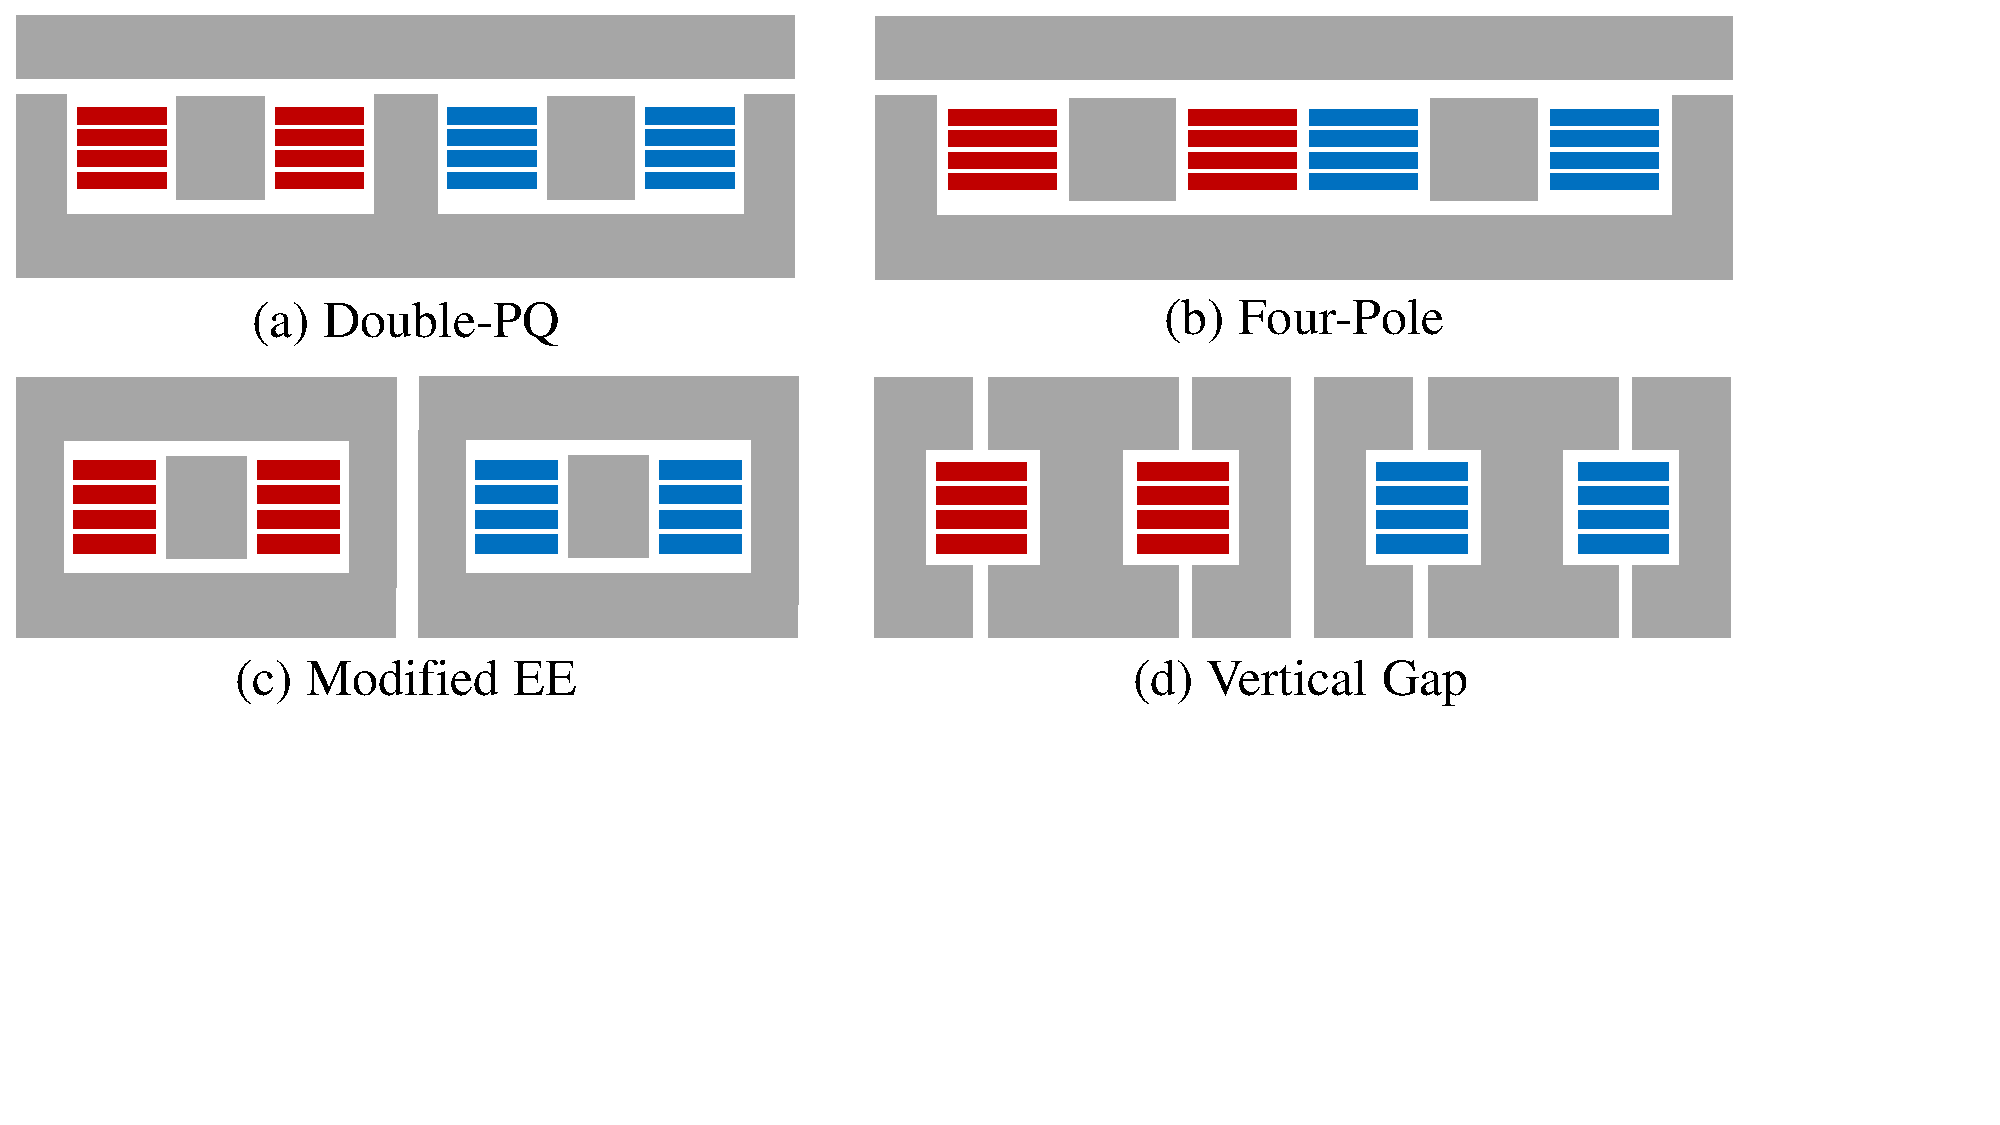
\includegraphics[page=1, trim = 0cm 7cm 4.5cm 0cm, clip, width=\columnwidth]{figures/IPEC_Figures_PowerPoint.pdf}
  \caption{Structure of the studied cores in side-view if cut through the middle. First winding in red, second winding in blue.} %ToDo: Show without dual air-gap?
  \label{fig:Core_Drawings}
\end{figure}
Four different geometries, two coupled, and two uncoupled ones, were compared for this work as shown in Fig. \ref{fig:Core_Drawings}. The Double-PQ structure was originally introduced by \cite{wangPCBWindingBasedCoupled2023} and combines two EQ-cores placed next to each other. The four-pole structure is very similar but omits the central pole \cite{huaUltrathinCoupledInductor2021}. Both of these geometries were originally constructed with two pieces such that there is only an air-gap at the top. The dual air-gap shown in Fig. \ref{fig:Core_Drawings} is introduced in this work. % ToDo: Where can we see that? Maybe change
 The third geometry is basically an EE-Core but instead of one central gap, two gaps are used. Lastly, the vertical gap geometry proposed by \cite{schaferNovelHighlyEfficient2020} is investigated which can partly compensate the internal proximity effect. %A notable downside of the vertical gap is that it prohibits cooling with conductive materials from the top and bottom, which is usually a big advantage of planar inductors, due to the external flux in this area. 
\par All designs use a single turn with all six layers in parallel which is very different from their original designs. %Six layers were chosen due to the significantly cheaper manufacturing cost compared to higher layer counts. The inner layers have a thickness of \qty{70}{\um} while the outer ones have only \qty{35}{\um}, due to the tight spacing of the selected gate-driver which required a \qty{35}{\um} outer layer at the selected manufacturer to meet clearance constraints. 
Designs with more than one turn were not considered because the desired inductance and coupling-factor could not be achieved in that case due to fringing. % ToDo: Explain

\paragraph{Material limitations}
TDK's PC200 was selected for this design as it exhibits very low loss in the range of \qtyrange{1}{4}{\MHz}. However, the performance of PC200 significantly degrades for a field strength $\sbl{Hdc} > \qty{50}{A/m}$ and at $\sbl{Hdc} > \qty{100}{A/m}$ its losses double%\footnote{This effect is even more pronounced in NiZn materials which can be permanently damaged by large fields.} 
\cite{tdkHighFrequencyLowLossFerrite}. Therefore, the inductor was designed with a maximum \sbl{Hdc} of \qty{40}{A/m} to have some margin.

\paragraph{Positive vs negative coupling}
\begin{figure}
    \centering
    %\resizebox{0.9\columnwidth}{!}{\input{figures/Python/current_ripple_plot.pgf}}
    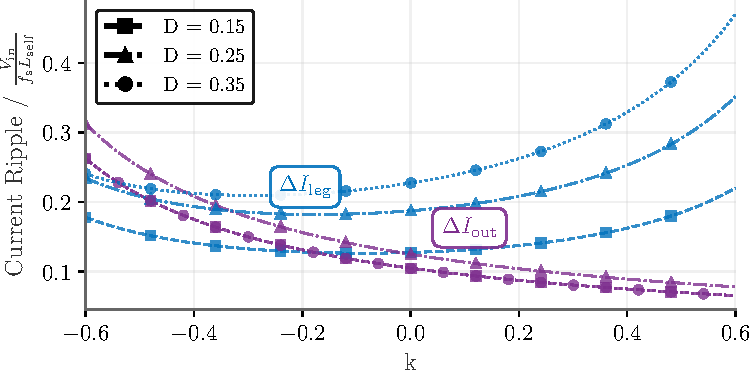
\includegraphics[width=0.95\columnwidth]{figures/Python/current_ripple_plot.pdf}
    \caption{Peak-to-peak leg and output current ripple in dependency of the coupling factor for different duty cycle. For $\sbl{D}=0.15$ and $\sbl{D}=0.35$ the output current ripple is identical so the curves overlap.}
    \label{fig:OutputAndLegRipple}
\end{figure}
\begin{figure}
  \includegraphics[page=3, trim = 0cm 1cm 3.5cm 0cm, clip, width=\columnwidth]{figures/IPEC_Figures_PowerPoint.pdf}
  \caption{Flux-Distribution for negative and positive coupling of otherwise identical designs for a DC phase current of \qty{40}{\A} and \qty{100}{\A} of ripple.}
  \label{fig:Fluxposneg}
\end{figure}


Equation (\ref{eq:DeltaIout}) and (\ref{eq:DeltaIleg}) are plotted in Fig. \ref{fig:OutputAndLegRipple} for positive and negative coupling-factors. While a strong positive coupling decreases \sbl{DeltaIout} it increases \sbl{DeltaIleg}. %This is intuitive when looking at Equation (\ref{eq:LoutandLmfromk}): A positive coupling factor shifts inductance from the magnetizing to the output inductance, resulting in lower output current ripple but higher magnetizing current ripple. This means positive coupling require a larger \sbl{Lself} to achieve the same \sbl{Ion} if all other parameters remain the same. \par
Overall, positive coupling is slightly beneficial from an electrical point of view as it reduces the output ripple. The higher \sbl{DeltaIleg} requires a larger \sbl{Lself} resulting in even lower \sbl{DeltaIout}. However, there is a very notable difference in the flux distribution as shown in Fig. \ref{fig:Fluxposneg}: For negative coupling, the two windings generate an opposing magnetomotive force at DC, resulting in a low flux that circulates through the outer air-gaps. For positive coupling, the two magnetomotive forces are driving a DC-flux in the same direction causing a large flux that only circulates between the two windings where the reluctance is much lower. The peak flux-density is almost three times larger for positive coupling and as the core should be designed with respect to the \sbl{Hdc} limit, this means thicker top and bottom areas would be needed. Therefore, negative coupling is selected for this application\footnote{Note that for lower frequency materials which are less affected by DC flux, the picture would change: Those designs would likely benefit from positive coupling as the flux-density at the fundamental is reduced.}. %For the fundamental (and all other odd harmonics), the flux-paths are swapped compared to DC (and even harmonics) as shown in Fig. \ref{fig:Fluxposneg} (c) and (d).

\paragraph{Simulation Process}
For the simulation, the open-source 2D FEM software FEMM was used due to its high speed and easy integration with Matlab. As the core-structures are neither planar nor axisymmetric, the designs were first transformed to a planar structure. All cross-sectional areas are kept the same and the depth of the design is determined by the length of the winding. % \\ For validation, the design was also transformed into an axisymmetric structure (neglecting the effects of coupling). This has the advantage that the current distribution and consequently copper-loss is closer to reality at the expense of less-precise core-loss.

\paragraph{Split air-gap and optimized windings}
\begin{figure}
  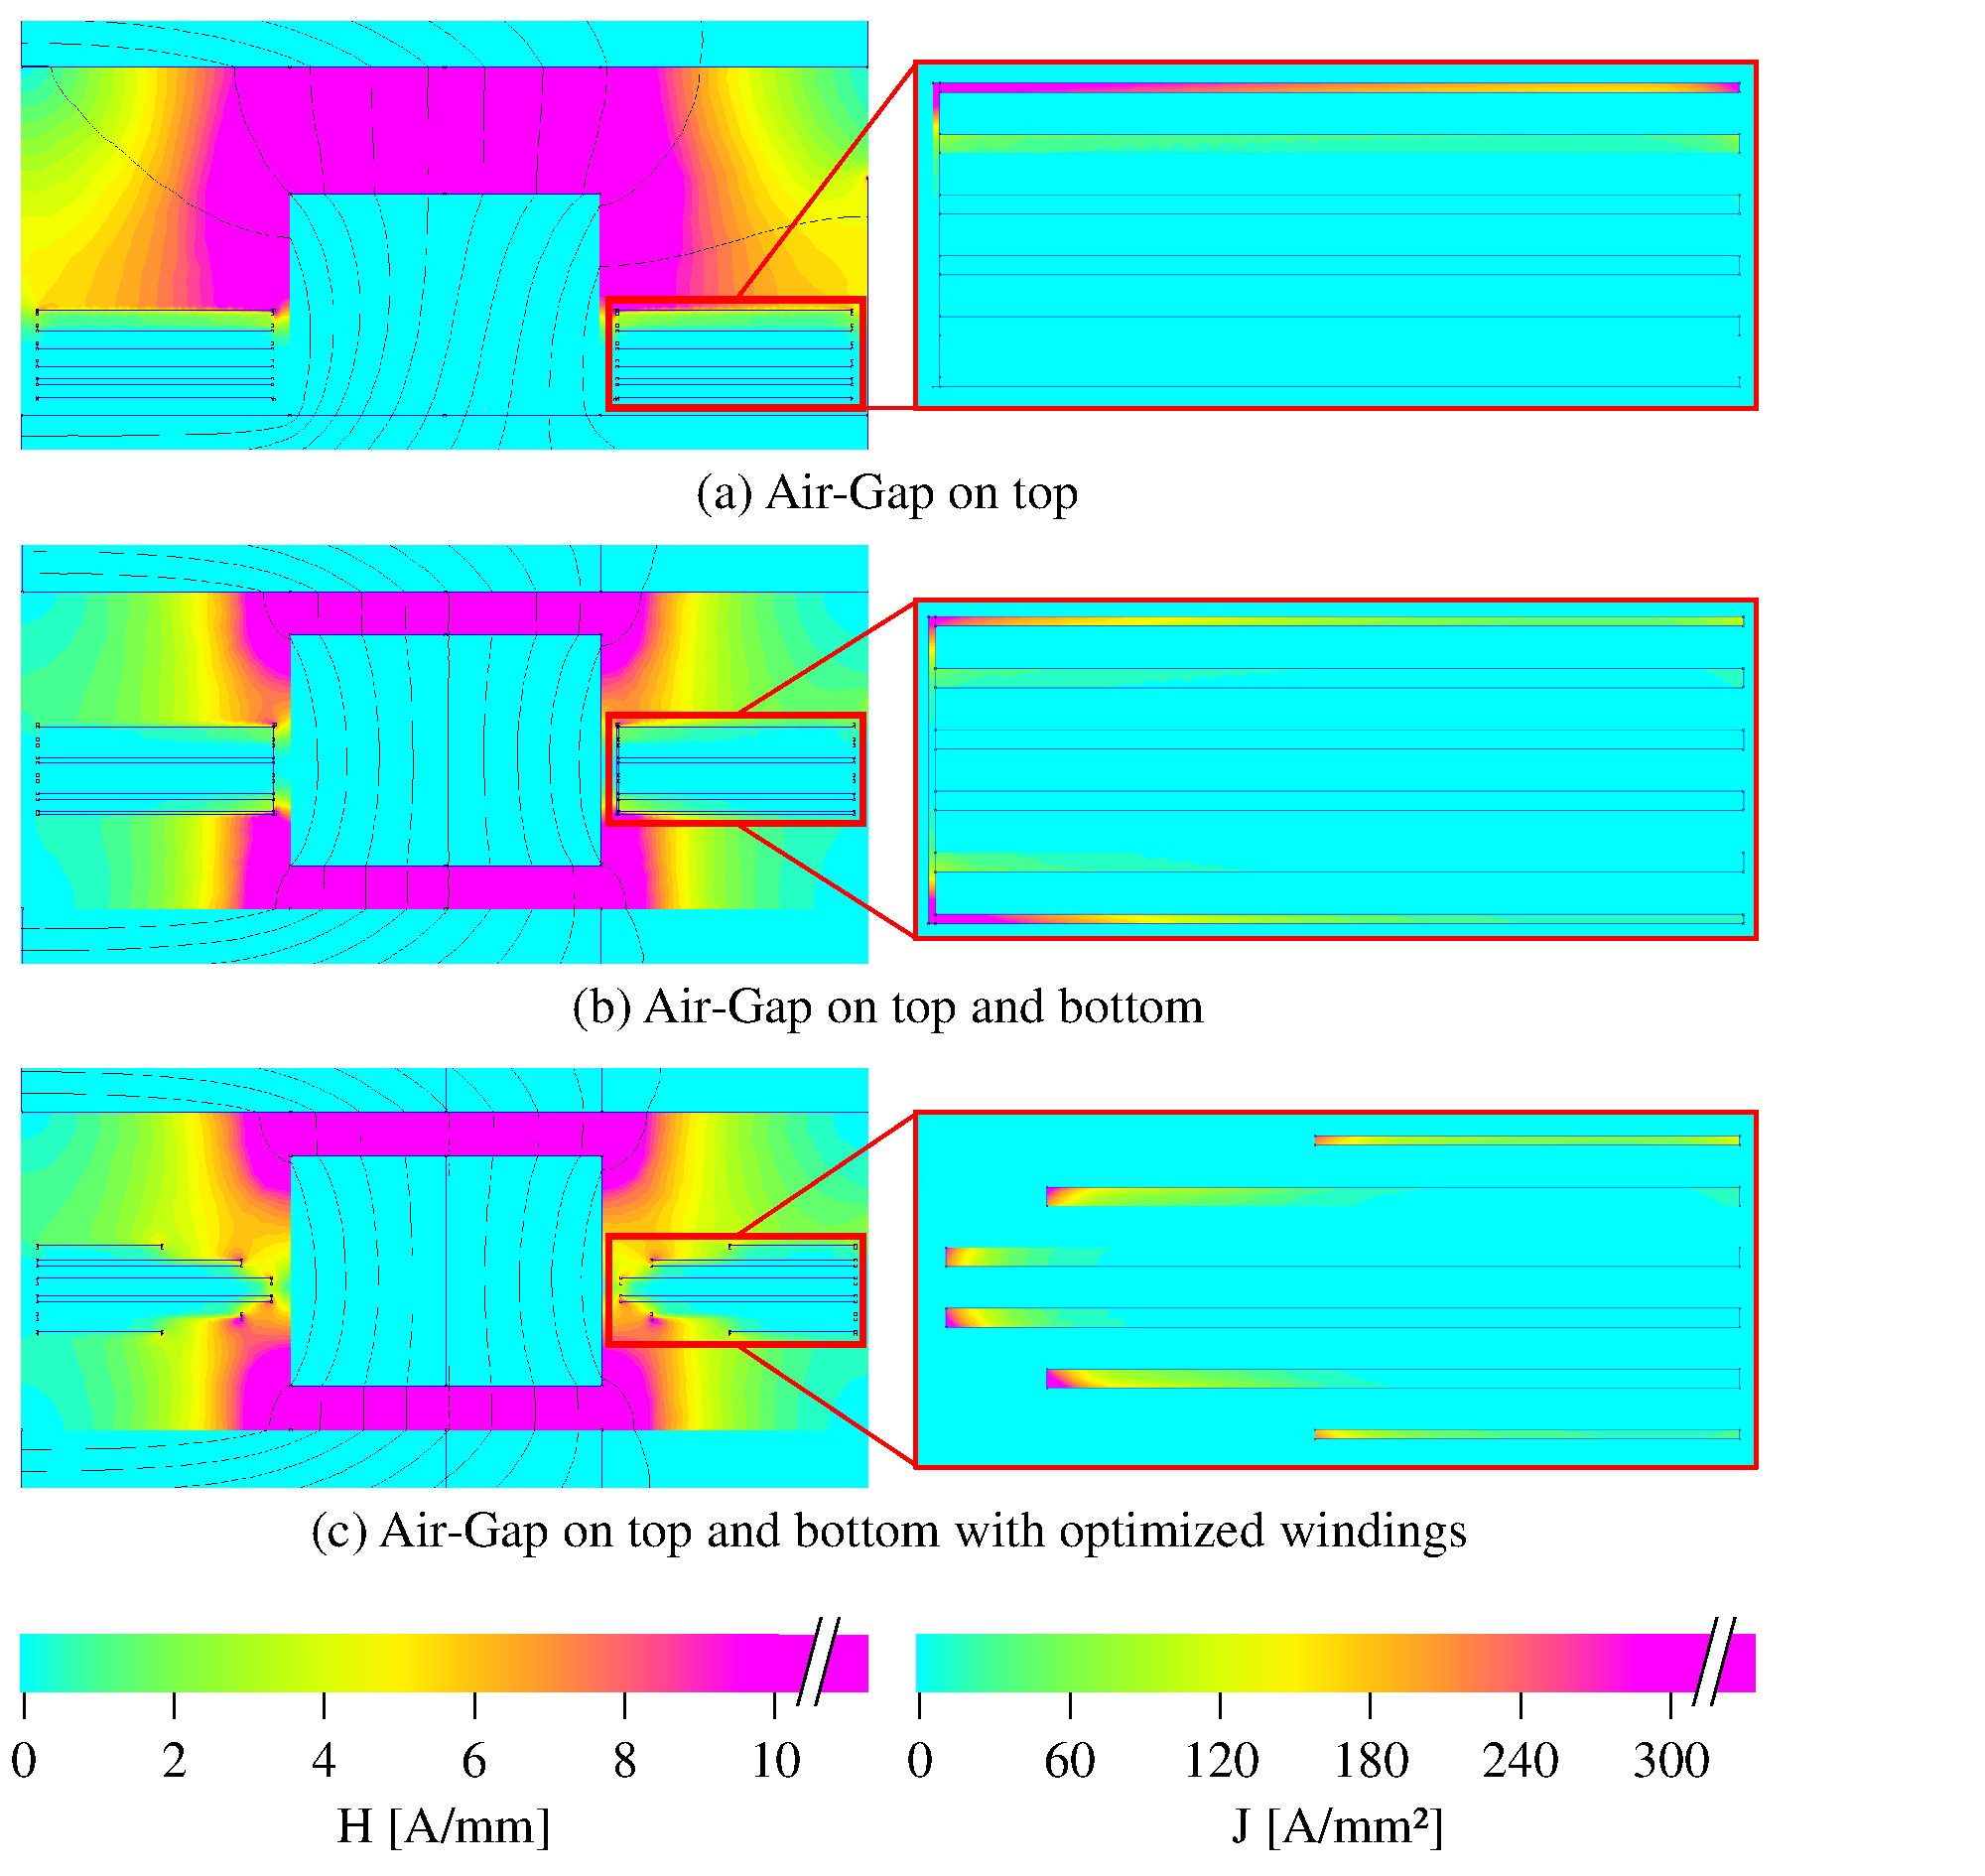
\includegraphics[page=1, trim = 0cm 0cm 3cm 0cm, clip, width=\columnwidth]{figures/IPEC_Figure_AirGap.pdf}
  \caption{Field and current distribution for different approaches. Because all layers are in parallel the current crowds in areas of large field-strength. By splitting the gap, the field gets distributed more evenly and the current distribution improves. Utilizing a smaller width for the outer layers, i.e. moving the copper away from the high-flux areas distributes the current even better.}
  \label{fig:OptimizedGap}
\end{figure}

\begin{table}
  \caption{Comparison of the size and loss of the optimized pillar and windings for the four-pole design.}
  \label{tab:OptimizationPQ}
  \centering
  \begin{tblr}{
      colspec={Xll},
      row{1}={font=\bfseries},
      column{1}={font=\itshape},
      row{even}={bg=gray!10},
    }
    & {Volume [\unit{\cubic\cm}]} & {Copper Loss [\unit{\W}]} \\
    \toprule
    Original design & 5.8 & 7.0 \\
    Air-Gap on top and bottom & 5.5 & 5.7 \\
    Air-Gap on top and bottom, curved windings & 5.3 & 5.0 \\
    \bottomrule
  \end{tblr}
\end{table}

The external proximity effect caused by the air-gap plays an important role for the current distribution and consequently the losses of this high-frequency inductor. The field-strength at the top of the windings is large and almost zero at the bottom. As a result, the AC current is only flowing in the top layers. By centering the pillar vertically in the window such that there is an equal air-gap on the top and on the bottom, the field-strength is distributed much more uniformly and current flows in the top and bottom layers. This results in a \qty{20}{\percent} reduction in losses, which can be reduced even further by using curved windings as shown in Table \ref{tab:OptimizationPQ}.

% \paragraph{Inductor Design Process}
% %Using a brute-force algorithm was deemed impossible due to the many free variables with the custom design. Instead, 
% A manual optimization was conducted for each structure. The desired switching-frequency was fixed to \qty{1.5}{\MHz} for full-load operation, the coupling-factor to -0.3, %ToDo: Explain why!
%  and the winding with to \qty{3}{\mm} as this showed a good balance between size and losses. The cross-sectional areas were designed to result in $\sbl{Hdc} \leq \qty{40}{\A\per\m}$ and the air-gaps are defined by desired inductance (i.e. switching frequency) and coupling-factor. The spacing between \ac{pcb} and top/bottom of the core is the only free variable and has to be chosen for a compromise between size and efficiency.

% \begin{figure}
%   \centering
%   % This file was created by matlab2tikz.
%
\definecolor{mycolor1}{rgb}{0.00000,0.44700,0.74100}%
%
\begin{tikzpicture}

\begin{axis}[%
width=0.8\columnwidth,
height=0.35\columnwidth,
at={(0\columnwidth,0\columnwidth)},
scale only axis,
xmin=0.2,
xmax=2,
xlabel style={font=\color{white!15!black}},
xlabel={Spacing [mm]},
ymin=4.5,
ymax=7.5,
ylabel style={font=\color{white!15!black}},
ylabel={Copper-Loss [W]},
axis background/.style={fill=white},
xmajorgrids,
ymajorgrids
]
\addplot [color=mycolor1, mark=o, mark options={solid, mycolor1}, forget plot]
  table[row sep=crcr]{%
0.2	7.13296642485744\\
0.4	6.24346547710337\\
0.6	5.71549329037772\\
0.8	5.37601200977181\\
1	5.15029927094516\\
1.2	5.00087651688349\\
1.4	4.89772868492222\\
1.6	4.83930849566333\\
1.8	4.80515358408807\\
2	4.7881839177051\\
};
\addplot[mark=*] coordinates {(1.2, 5.00087651688349)} node[pin=30:{Design point}]{} ;
\end{axis}
\end{tikzpicture}%
%   \caption{Spacing between PCB and core vs. loss and inductor volume for the four-pole core (with curved windings and centered pillar). The distance between the PCB and the side air-gap core is fixed to \qty{0.2}{\mm} and the distance between PCB and bottom is varied. The pillar is always centered between top and bottom.}
%   \label{fig:fourPole_spacingVsLoss}
% \end{figure}

\paragraph{Vertical Air-Gap}
The design with vertical air-gap showed a significantly lower loss compared to a traditional horizontal gap while having a much lower volume. This confirms the results from \cite{schaferNovelHighlyEfficient2020}. The main downside of this design is the significant external field on top and bottom of the inductor, making cooling difficult as no conductive material can be placed on top or bottom of the core. %, eliminating one of the typical advantages of planar inductors: The large area for cooling. Cooling from the side is proposed by \cite{schaferNovelHighlyEfficient2020} by having copper extending to the outside of the core where a heatsink can be attached but this is much less convenient and requires additional space.

\paragraph{Comparison of Core Structures}
Table \ref{tab:InductorComparison} compares the different core structures for a design with $\sbl{fs}=\qty{1.5}{\MHz}$ at $\overline{\sbl{iout}} = \qty{80}{\A}$ and $\sbl{k} = -0.3$. This coupling factor was chosen because it allows the use of small air gaps at the pillar which reduces copper losses due to the smaller external field while still not increasing \sbl{DeltaIout} too much. The cross-sectional areas were designed to result in $\sbl{Hdc} \leq \qty{40}{\A\per\m}$. All designs except the one with vertical gap use the optimized curved windings. The four-pole structure showed the lowest losses and volume and was chosen for the implementation. The inductor design is shown in Fig. \ref{fig:Four-Pole-3d}.

\begin{table}
  \caption{Comparison of the size and loss of the different core structures for \qty{1.5}{\MHz} respecting the \sbl{Hdc} limit. The Four-Pole structure shows the lowest losses and volume.}
  \label{tab:InductorComparison}
  \centering
  \begin{tblr}{
      colspec={lXXXX},
      row{1}={font=\bfseries},
      column{1}={font=\itshape},
      row{even}={bg=gray!10},
    }
    & {Total Area [\unit{\cm\squared}]} & {Height [\unit{\cm}]} & {Volume [\unit{\cubic\cm}]} & {Copper Loss [\unit{\W}]} \\
    \toprule
      Four-Pole & 5.5 & 0.9 & 5.3 & 5.0 \\
      Double PQ & 6.2 & 0.9 & 5.5 & 5.2 \\
      Vertical gap & 8.0 & 0.7 & 5.8 & 5.6 \\
      UU core & 8.1 & 1.1 & 8.9 & 6.0 \\
    \bottomrule
  \end{tblr}
\end{table}

\begin{figure}
  \centering
  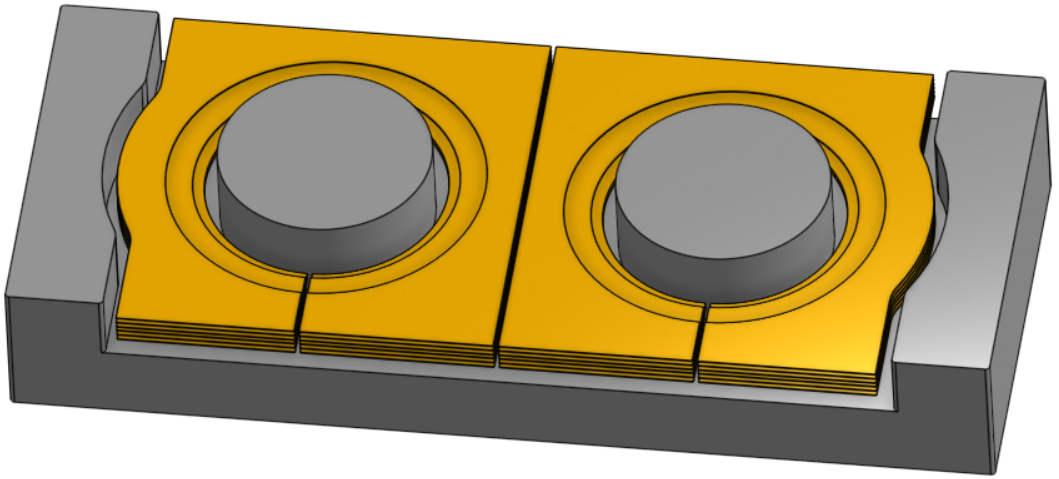
\includegraphics[width=0.6\columnwidth]{figures/Four-Pole-3d.png}
  \caption{Final design of the four-pole inductor; top-piece not shown.}
  \label{fig:Four-Pole-3d}
\end{figure}


\section{Experimental prototype}
\begin{figure}
  \centering
  \includegraphics[page=2, trim = 0cm 0cm 3cm 0cm, clip, width=0.8\columnwidth]{figures/IPEC_Figures_PowerPoint.pdf}
  \caption{Fully assembled prototype (without heatspreader).  The converter area shown in orange is 45 x 29 x \qty{9.5}{\mm}. Outside of this area only the connectors for power and programming are placed as well as a protection diode and the programming resistors. ToDo: White Background and place match next to it.}
  \label{fig:PrototypePicture}
\end{figure}

\begin{table}
  \caption{Overview of the main hardware components.}
  \label{tab:Hardware}
  \centering
  \begin{tblr}{
      colspec={ll},
      row{1}={font=\bfseries},
      row{even}={bg=gray!10},
    }
    Component & Part \\
    \toprule
    $\mathrm C_\mathrm{in}$         & 44x \qty{2.2}{\uF} \qty{100}{\V} X7R (\qty{20}{\uF} at \qty{48}{\V})  \\
    $\mathrm C_\mathrm{out}$        & 16x \qty{2.2}{\uF} \qty{100}{\V} X7R (\qty{33}{\uF} at \qty{12}{\V}) \\
    GaN-FETs          & Infineon IGC025S08S1            \\
    Gate Driver       & Analog Devices LT8418           \\
    Microcontroller   & Texas Instruments F280049C      \\
    Aux. Power Supply & Texas Instruments TPSM365R6     \\
    Current Sensor    & Allegro ACS37220                \\  
    \bottomrule
  \end{tblr}
\end{table}


The assembled prototype is shown in Fig. \ref{fig:PrototypePicture}. The boxed volume of just \qty{12.4}{\cubic\cm} results in a power density of \qty{80}{\kW\per\liter} (\qty{1300}{\W\per\cubic\inch}). It's main hardware components are listed in table \ref{tab:Hardware}. Two parallel low side transistors per phase are used as the converter operates at a low duty cycle. To minimize the stray inductance, the decoupling capacitors for the half-bridges were connected to the devices with a so-called vertical power-loop layout which uses the first inner layer as a return path \cite{reuschUnderstandingEffectPCB2014}. In contrast to other designs, the large onboard capacitance allows the converter to operate without any additional off-board capacitance. \par
The converter operates over the entire range as expected. The efficiency is shown in Fig. \ref{fig:Efficiency} which reaches its maximum of \qty{96.3}{\percent} at around \qty{550}{\W}. As expected, the efficiency significantly drops for each frequency once a certain power is exceeded. This is caused by the operation in \ac{tcm}: The leg-current ripple is proportional to the switching frequency and to achieve soft-switching, a certain negative current is required prior to the turn-off of the low-side switch, otherwise the voltage at the switching node will not rise fast enough to yield soft-switching. As the output current rises, the negative current rises and at some point, soft-switching is lost. %However, as long as there is some negative current the switch-node potential still rises within the dead time such that the turn-on losses are reduced. This explains the gradual decrease of the efficiency. 
To use the converter in a real application, a variable switching frequency is required. The expected resulting efficiency curve is indicated in Fig. \ref{fig:Efficiency}.

\begin{figure}
  \centering
  %% Matlab Colors
\definecolor{mycolor1}{rgb}{0.00000,0.44700,0.74100}%
\definecolor{mycolor2}{rgb}{0.85000,0.32500,0.09800}%
\definecolor{mycolor3}{rgb}{0.92900,0.69400,0.12500}%
\definecolor{mycolor4}{rgb}{0.49400,0.18400,0.55600}%
\definecolor{mycolor5}{rgb}{0.46600,0.67400,0.18800}%
\definecolor{mycolor6}{rgb}{0.30100,0.74500,0.93300}%

\begin{tikzpicture}
    \begin{axis}[%
        axis y line*=left,
        width=\columnwidth,
        height=0.6\columnwidth,
        xmin=0,
        xmax=1000,
        ymin = 0.9,
        ymax = 0.98,
        xlabel={\sbl{Pout} [W]},
        ylabel={Efficiency},
        yticklabel={\pgfmathparse{\tick*100}\pgfmathprintnumber{\pgfmathresult}\%},
        xmajorgrids,
        xminorgrids,
        minor x tick num=1,
        ymajorgrids,
        yminorgrids,
        minor y tick num=1,
        legend style={at={(0.5,-0.3)}, anchor=north, legend cell align=left, align=left, draw=white!15!black},
        legend columns=3,
        cycle list name=mark list*
    ]
        \addplot+ [smooth, color=mycolor1, mark options={solid, mark size=1.5pt, mycolor1}]
        table[row sep=crcr]{%
62.9	0.691694257\\
125.5	0.815818548\\
188.0	0.867678959\\
250.2	0.896092267\\
312.2	0.913584221\\
373.9	0.925145996\\
435.3	0.93331475\\
496.4	0.939204148\\
557.1	0.943657677\\
617.3	0.946993756\\
676.9	0.949462788\\
735.9	0.951215098\\
794.0	0.952391805\\
850.7	0.953146007\\
905.1	0.953529288\\
954.3	0.953652443\\
997.8	0.952362317\\
1039.1	0.948949772\\
        };
        \addlegendentry{\qty{1.25}{\MHz}}

        \addplot+ [smooth, color=mycolor2, mark options={solid, mark size=1.5pt, mycolor2}]
        table[row sep=crcr]{%
61.7	0.742108935\\
123.1	0.85041111\\
184.2	0.893615989\\
245.0	0.916766467\\
305.3	0.93057418\\
365.3	0.939723701\\
424.7	0.946047092\\
483.5	0.950520936\\
541.7	0.953613238\\
598.6	0.955864976\\
653.7	0.957448367\\
704.7	0.958501088\\
749.6	0.95826356\\
792.8	0.955006505\\
829.8	0.948969556\\
        };
     \addlegendentry{\qty{1.5}{\MHz}}

        \addplot+ [smooth, color=mycolor3, mark options={solid, mark size=1.5pt, mycolor3}]
        table[row sep=crcr]{%
62.1	0.808207945\\
123.7	0.892705101\\
184.8	0.924369748\\
245.2	0.940517737\\
305.0	0.950394167\\
363.6	0.95630787\\
420.3	0.960332694\\
473.4	0.963192056\\
520.6	0.963357083\\
565.4	0.958645597\\
604.5	0.949556994\\
640.3	0.942556825\\
        };
        \addlegendentry{\qty{2}{\MHz}}

        \addplot+ [smooth, color=mycolor4, mark options={solid, mark size=1.5pt, mycolor4}]
        table[row sep=crcr]{%
59.5	0.841743314\\
118.1	0.911878282\\
175.6	0.937486654\\
231.5	0.950322289\\
284.5	0.958559348\\
331.7	0.96159309\\
375.4	0.955384185\\
414.1	0.942270059\\
442.7	0.927589675\\
        };
        \addlegendentry{\qty{2.5}{\MHz}}

        \addplot+ [smooth, color=mycolor5, mark options={solid, mark size=1.5pt, mycolor5}]
        table[row sep=crcr]{%
57.2	0.856371361\\
112.7	0.920470319\\
165.5	0.943988136\\
212.8	0.95387305\\
255.4	0.94690003\\
293.2	0.927676538\\
316.8	0.902598143\\
        };
        \addlegendentry{\qty{3}{\MHz}}

        \addplot+ [smooth, color=mycolor6, mark=none]
        table[row sep=crcr]{%
213.23	0.95387305\\
332.12	0.96159309\\
520.87	0.9634\\
749.68	0.9583\\
954.41	0.953652443\\
        };
        \addlegendentry{Max}

\end{axis}
\end{tikzpicture}%
  \caption{Efficiency of the prototype for $\sbl{Vin}=\qty{48}{\V}$ and $D=0.25$.}
  \label{fig:Efficiency}
\end{figure}

\section{Conclusion}
Preliminary results show that the buck converter with negatively coupled, single turn inductors is capable of achieving very high power density and efficiency for \qty{48}{\V} to \qty{12}{\V} conversion. Utilizing the transformer model, compact equations for the key electrical parameters were derived in dependency of the coupling factor. It was shown that positive and negative coupling are ambivalent in their electrical parameters but negative coupling creates a much lower DC flux which is important for high-frequency materials. Utilizing a dual air-gap and optimized windings, losses could be decreased significantly. \par
The final paper will also include a thermal analysis of the converter. The maximum achievable output power is expected to be higher than currently shown as the cooling system is not at capacity. It will also include more detailed measurements of the efficiency with a fixed conversion ratio instead of fixed duty cycle as well as efficiency in boost-mode. Furthermore, a more detailed analysis of the losses will be presented, comparing the different sources of losses in simulation with measurements from the prototype.

\bibliographystyle{IEEEtranNDoi}
\bibliography{Paper_Bibliography}

\end{document}

% https://ipec2026.org/regular-session/ 

% The extended summary should clearly define the salient concepts
% and novel features of the work. Be sure to mention past or
% previous works to distinguish your originality from them. The
% extended summary should be up to 4 pages except Reference,